\chapter{Advanced Matching and Rewriting}\indexmain{advanced matching and rewriting}
\label{chapadvanced}

The advanced \emph{modifiers} introduced in the following section allow to annotate patterns or actions with keywords which restrict what graph patterns are accepted as matches (some of them independent of the rewrite part, some of them depending on the rewrite specification).
But first the advanced \emph{matching} constructs are introduced in this section, before they are elaborated on in a later section:
they allow to request more fine grain or more dynamically what types to match, as well as allowing to specify a match from a storage.
Followed by the advanced \emph{rewrite} constructs which are handled in the same way (introduction here, then elaboration in a later section);
these enable the specification of retyping (relabeling) and copying, as well as node merging and edge redirection.

\begin{rail}
AdvancedNodeTypeConstructs : ( NodeType (TypeConstraint | StorageAccess | Retyping | Merging) | CopyOperator);
\end{rail}\ixnterm{AdvancedNodeTypeConstructs}

Specifies a node of type \emph{NodeType},
constrained in type with a \emph{TypeConstraint}\indexmain{type constraint} (see Section~\ref{sec:typeconstr}, \emph{TypeConstraint}),
or bound by a storage access (see \ref{sub:storageaccess}, \emph{StorageAccess}),
or retyped with a \emph{Reytping}\indexmain{retype} (see Section~\ref{sec:retype}, \emph{Retyping}),
or merged with a \emph{Merging}\indexmain{merge} (see Section~\ref{sec:merge}, \emph{Merging}).
Alternatively it may define a node having the same type and bearing the same attributes as another matched node (see Section~\ref{sec:copy}, \emph{CopyOperator}).
Type constraints are allowed in the pattern part only.
The CopyOperator and the Merging clause are allowed in the replace/modify part only.
The Retyping clause is a chimera which restricts the type of an already matched node when used on the LHS, and casts to the target type when used on the RHS, which is its primary use.

\begin{rail}
AdvancedEdgeTypeConstructs : ( EdgeType (TypeConstraint | StorageAccess | Retyping) | CopyOperator);
\end{rail}\ixnterm{AdvancedEdgeTypeConstructs}

The \emph{AdvancedEdgeTypeConstructs} specify an edge of type \emph{EdgeType} or a copy of an edge.
Type constraints\indexmain{type constraint} are allowed in the pattern part only (see Section~\ref{sec:typeconstr}, \emph{TypeConstraint}); 
the same holds for the storage access (see \ref{sub:storageaccess}, \emph{StorageAccess}).
The CopyOperator and the Redirect clause are allowed in the replace/modify part only (see Section~\ref{sec:copy}, \emph{CopyOperator}, see Section~\ref{sec:redirect}, \emph{Redirect}).
The Retyping clause is a chimera which restricts the type of an already matched edge when used on the LHS, and casts to the target type when used on the RHS (its primary use).
Furthermore edges may be redirected, this is shown in Section~\ref{sec:redirect}, \emph{Redirection}.


%%%%%%%%%%%%%%%%%%%%%%%%%%%%%%%%%%%%%%%%%%%%%%%%%%%%%%%%%%%%%%%%%%%%%%%%%%%%%%%%%%%%%%%%%%%%%%%%
\section{Rule and Pattern Modifiers}\indexmain{modifier}
\label{sct:patternmodifier}

\begin{rail}
  TestModifier: (() | 'exact' | 'induced') ;
  RuleModifier: (TestModifier | 'dpo' | 'dangling' | 'identification' ) ;
\end{rail}\ixkeyw{exact}\ixkeyw{induced}\ixkeyw{dpo}\ixkeyw{dangling}\ixkeyw{identification}

By default \GrG\ performs rewriting according to \indexmain{SPO}SPO semantics as explained in Section~\ref{rule:morphismr}.
This behaviour can be changed with \newterm{pattern modifiers} and \newterm{rule modifiers} (and the other advanced rewrite constructs introduced in the following sections which spoil the theoretical foundation but are highly useful in practice).
Such modifiers add certain conditions to the applicability of a pattern.
The idea is to match only parts of the host graph that look more or less exactly like the pattern.
The level of ``exactness'' depends on the choosen modifier.
A pattern modifier in front of the \texttt{rule}/\texttt{test}-keyword is equivalent to one modifier-statement inside the pattern containing all the specified nodes (including anonymous nodes).
Table \ref{tbl:rules:patternmodifiers} lists the pattern modifiers with their semantics, table \ref{tbl:rules:rulemodifiers} lists the rule only modifiers with their semantics.
Example \ref{ex:rules:modifiers} explains the modifiers by small toy-graphs.

\begin{table}[htbp]
    \begin{tabularx}{\linewidth}{l|X}
        \bf Modifier & \bf Meaning \\\hline
        \texttt{exact} & Switches to the most restricitive mode. An exactly-matched node is matched, if all its incident edges in the host graph are specified in the pattern.\\
        \texttt{induced} & Switches to the induced-mode, where nodes contained in the same \texttt{induced} statement require their induced subgraph within the host graph to be specified, in order to be matched. In particular this means that in general \texttt{induced(a,b,c)} differs from \texttt{induced(a,b); induced(b,c)}.\\
    \end{tabularx}
    \caption{Semantics of pattern modifiers}
    \label{tbl:rules:patternmodifiers}
\end{table}

\begin{table}[htbp]
    \begin{tabularx}{\linewidth}{l|X}
        \bf Modifier & \bf Meaning \\\hline
        \texttt{dpo} & Switches to DPO semantics \indexmainsee{DPO}{double-pushout approach}. This modifier affects only nodes that are to be deleted during the rewrite. DPO says---roughly spoken---that implicit deletions must not occur by all means. To ensure this the dangling condition (see \texttt{dangling} below) and the identification condition (see \texttt{identification} below) get enforced (i.e. \texttt{dpo = dangling + identification}). In contrast to \texttt{exact} and \texttt{induced} this modifier applies neither to a pattern as such (can't be used with a \texttt{test}) nor to a single statement but only to an entire rule. See Corradini et al.\cite{dpoapproach} for a DPO reference.\\
		\texttt{dangling} & Ensures the dangling condition \indexmain{dangling condition}. This modifier affects only nodes that are to be deleted during the rewrite. Nodes going to be deleted due to the rewrite part have to be specified exactly (with all their incident edges, \texttt{exact} semantics) in order to be matched. As with \texttt{dpo}, this modifier applies only to rules.\\
		\texttt{identification} & Ensures the identification condition \indexmain{identification condition}. This modifier affects only nodes that are to be deleted during the rewrite. If you specify two pattern graph elements to be homomorphically matched but only one of them is subject to deletion during rewrite, those pattern graph elements will never actually be matched to the same host graph element. As with \texttt{dpo}, this modifier applies only to rules.\\
    \end{tabularx}
    \caption{Semantics of rule only modifiers}
    \label{tbl:rules:rulemodifiers}
\end{table}

\begin{note}
    Internally all the modifier-annotated rules are resolved into equivalent rules in standard SPO semantics.
    The semantics of the modifiers is mostly implemented by NACs.
    In particular you might want to use such modifiers in order to avoid writing a bunch of NACs yourself.
    The number of internally created NACs is bounded by $\mathcal{O}(n)$ for \texttt{exact} and \texttt{dpo} and by $\mathcal{O}(n^2)$ for \texttt{induced} respectively, where $n$ is the number of specified nodes.
\end{note}

\begin{figure}[htbp]
\begin{example}
    \label{ex:rules:modifiers}
    \begin{center}
        \begin{tabularx}{\linewidth}{llX}
            \bf Host Graph & \bf Pattern / Rule & \bf Effect \\\hline
            & & \\
            \begin{tabular}[c]{@{}l}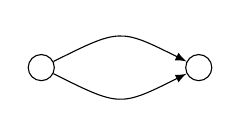
\begin{tikzpicture}
                \tikzstyle{every node}=[circle]
                \node[draw] (n1) at (0,0) {};
                \node[draw] (n2) at (2,0) {};

                \draw[-latex] (n1) .. controls +(+1,+0.5) .. (n2) {};
                \draw[-latex] (n1) .. controls +(+1,-0.5) .. (n2) {};
            \end{tikzpicture}\end{tabular} &
                \begin{tabular}[c]{@{}l}\texttt{\{ .\ --> .; \}}\end{tabular} &
                Produces no match for \texttt{exact} nor \texttt{induced}\\
            & & \\
            \begin{tabular}[c]{@{}l}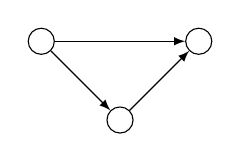
\begin{tikzpicture}
                \tikzstyle{every node}=[circle]
                \node[draw] (n1) at (0,0) {};
                \node[draw] (n2) at (2,0) {};
                \node[draw] (n3) at (1,-1) {};

                \draw[-latex] (n1) -- (n2) {};
                \draw[-latex] (n1) -- (n3) {};
                \draw[-latex] (n3) -- (n2) {};
            \end{tikzpicture}\end{tabular} &
                \begin{tabular}[c]{@{}l}\texttt{\{ x:node --> y:node; \}}\end{tabular} &
                Produces three matches for \texttt{induced(x,y)} but no match for \texttt{exact(x,y)}\\
            & & \\
            \begin{tabular}[c]{@{}l}\begin{tikzpicture}
                \tikzstyle{every node}=[circle]
                \node[draw] (n1) at (0,0) {};

                \draw[-latex] (n1) .. controls +(+1,+0.5) and +(0,-1) .. (n1) {};
            \end{tikzpicture}\end{tabular} &
                \begin{tabular}[c]{@{}l}\texttt{\{ x:node; induced(x); \}}\end{tabular} &
                Produces no match\\
            & & \\
            \begin{tabular}[c]{@{}l}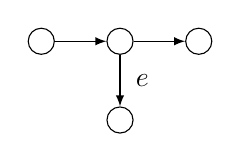
\begin{tikzpicture}
                \tikzstyle{every node}=[circle]
                \node[draw] (n1) at (0,0) {};
                \node[draw] (n2) at (1,0) {};
                \node[draw] (n3) at (2,0) {};
                \node[draw] (n4) at (1,-1) {};
    	c
                \draw[-latex] (n1) -- (n2) {};
                \draw[-latex] (n2) -- (n3) {};
                \draw[-latex] (n2) -- (n4) node[midway,right] {$e$};
            \end{tikzpicture}\end{tabular} &
                \begin{tabular}[c]{@{}l}\texttt{pattern\{ --> x:node --> ; \}}\\\texttt{modify\{ delete(x); \}}\end{tabular} &
                Produces no match in DPO-mode because of edge \texttt{e}\\
        \end{tabularx}
    \end{center}
\end{example}
\end{figure}


%%%%%%%%%%%%%%%%%%%%%%%%%%%%%%%%%%%%%%%%%%%%%%%%%%%%%%%%%%%%%%%%%%%%%%%%%%%%%%%%%%%%%%%%%%%%%%%%
\section{Static Type Constraint and Exact Dynamic Type}

In the following section we'll have a look at a language construct to statically constrain the types to match by excluding forbidden types and at a language construct which allows to require an element to be typed the same as another element or to create an element with the same exact dynamic type as another element.

%-----------------------------------------------------------------------------------------------
\subsection{Static Type Constraint}
\label{sec:typeconstr}
A static type constraint given at a node or edge declaration limits the types on which the pattern element will match.

\begin{rail}
  TypeConstraint: backslash ( '(' (TypeExpr + '+')  ')' | TypeExpr );
\end{rail}\ixnterm{TypeConstraint}
A \indexed{type constraint} is used to exclude parts of the \indexed{type hierarchy}. The operator \texttt{+} is used to create a union of its operand types. So the following pattern statements are identical:\\
\begin{center}
\begin{tabular}[c]{|ll|ll|}\hline
\begin{tabular}{l}\texttt{x:T \char"5C\ (T1 + $\cdots$ + T$n$);}\\\end{tabular} &&&
  \begin{tabular}{l}\texttt{x:T;} \\ \texttt{if \{!(\emph{typeof}(x) >= T1) \&\& $\cdots$} \\ \texttt{\ \ \ \ \&\& !(\emph{typeof}(x) >= T$n$)\}}\\\end{tabular} \\\hline
\end{tabular}
\end{center}

\begin{example}
\begin{tabularx}{\linewidth}{cX}
  \begin{tikzpicture}[baseline=(T.base)] \tt
    \begin{scope}[minimum size=0.5cm]
      \tikzstyle{every node}=[draw]
      \node (T)     at (1   ,4) {\texttt{T}};
      \node (T1)     at (1   ,3) {\texttt{T1}};
      \node (T2)     at (0   ,2) {\texttt{T2}};
      \node (T4)     at (0   ,1) {\texttt{T4}};
      \node (T3)     at (2   ,2) {\texttt{T3}};
    \end{scope}
    \draw[thick,-open triangle 45]  (T1) -> (T)  ;
    \draw[thick,-open triangle 45]  (T2) -> (T1)  ;
    \draw[thick,-open triangle 45]  (T3) -> (T1)  ;
    \draw[thick,-open triangle 45]  (T4) -> (T2)  ;
  \end{tikzpicture} &
  \parbox{\linewidth}{The type constraint \texttt{T\char"5C (T2+T3)} applied to the type hierarchy on the left side yields only the types \texttt{T} and \texttt{T1} as valid.}
\end{tabularx}
\end{example}

%-----------------------------------------------------------------------------------------------
\subsection{Exact Dynamic Type}\indexmainsee{exact dynamic type}{dynamic type}\indexmain{dynamic type}\label{sec:typeof}

\begin{rail}
  Type: TypeIdent | 'typeof' '(' NodeOrEdge ')' ;
\end{rail}\ixkeyw{typeof}\ixnterm{Type}
The type of a graph element may be given by a type identifier,
or a typeof denoting the exact dynamic type of a matched graph element.
The element declaration \texttt{el:typeof(x)} introduces a graph element of the type the host graph element \texttt{x} is actually bound to.
It may appear in the pattern or in the rewrite part.
If it is given in the pattern, the element to match must be of the same exact dynamic type as the element referenced in the \texttt{typeof}, otherwise matching will fail.
If is is given in the rewrite part, the element to create is created with the same exact dynamic type as the element referenced in the \texttt{typeof}; have a look at the next section for the big brother of this language construct, the \texttt{copy} operator, which is only applicable in the rewrite part.

\begin{example}
The following rule will add a reverse edge to a one-way street.
\begin{grgen}
rule oneway {
    a:Node -x:street-> y:Node;
    negative {
        y -:typeof(x)-> a;
    }
    replace {
        a -x-> y;
        y -:typeof(x)-> a;
    }
}
\end{grgen}
Remember that we have several subtypes of \texttt{street}. By the aid of the \texttt{typeof} operator, the reverse edge will be automatically typed correctly (the same type as the one-way edge). This behavior is not possible without the \texttt{typeof} operator.
\end{example}


%%%%%%%%%%%%%%%%%%%%%%%%%%%%%%%%%%%%%%%%%%%%%%%%%%%%%%%%%%%%%%%%%%%%%%%%%%%%%%%%%%%%%%%%%%%%%%%%
\section{Retyping and Copying}

In the following section we'll have a look at a language construct which retypes an element to another type
(either to a type statically given or the runtime type of another element),
changing the accessible attributes while keeping incident elements.
And at the copy operator which allows to create a new element of the runtime type of another matched element, transferring the attribute values.

%-----------------------------------------------------------------------------------------------
\subsection{Retyping} \label{sec:retype}
In addition to graph rewriting, \GrG\ allows graph relabeling\cite{Relabelling}, too; we prefer to call it retyping.
Nodes as well as edges may be retyped to a different type; attributes common to the initial and final type are kept.
The target type does not need to be a subtype or supertype of the original type.
Retyping is useful for rewriting a node but keeping its incident edges; without it you'd need to remember and restore those.
Syntactically it is specified by giving the original node enclosed in left and right angles.
\begin{rail}
  Retyping: '<' Ident '>';
\end{rail}\ixnterm{Retyping}

\begin{table}[htbp]
\centering
\begin{tabularx}{\linewidth}{lllX}
  \textbf{Pattern (LHS)} & \textbf{Replace (RHS)} & \textbf{$r: L \longrightarrow R$} & \textbf{Meaning} \\ \hline
  \texttt{x:N1;} & \texttt{y:N2<x>;}          & $r:\lhs.x \mapsto \rhs.x$ & Match \texttt{x}, then retype \texttt{x} from \texttt{N1} to \texttt{N2} and bind name \texttt{y} to retyped version of \texttt{x}.\\
  \texttt{e:E1;} & \texttt{f:E2<e>;}          & $r:\lhs.e \mapsto \rhs.e$ & Match \texttt{e}, then retype \texttt{e} from \texttt{E1} to \texttt{E2} and bind name \texttt{f} to the retyped version of \texttt{e}.\\
\end{tabularx}
\caption{Retyping of matched nodes and edges}
\label{rule:retyping_graphlets}
\end{table}

\indexmain{retyping}Retyping enables us to keep all adjacent nodes and all attributes stemming from common super types of a graph element while changing its type (table~\ref{rule:retyping_graphlets} shows how retyping can be expressed both for nodes and edges).
Retyping differs from a \indexedsee{type cast}{retyping}: During replacement both of the graph elements are alive.
  Specifically both of them are available for evaluation, a respective evaluation could, e.g., look like this:
  \begin{grgenlet}
eval {
  y.b = ( 2*x.i == 42 );
  f.a = e.a;
}
  \end{grgenlet}
Furthermore the source and destination types need \emph{not} to be on a path in the directed \indexed{type hierarchy} graph, rather their relation can be arbitrary.
However, if source and destination type have one ore more common super types, then the respective attribute values are adopted by the retyped version of the respective node (or edge).
The edge specification as well as \emph{ReplaceNode} supports retyping.
In Example~\ref{ex:rule:SomeRule} node \texttt{n5} is a retyped node stemming from node \texttt{n1}.
Note, that---conceptually---the retyping is performed \emph{after} the SPO conforming rewrite.

\begin{example}
The following rule will promote the matched city \texttt{x} from a \texttt{City} to a \texttt{Metropolis} keeping all its incident edges/streets,
with exception of the matched street \texttt{y}, which will get promoted from \texttt{Street} to \texttt{Highway}, keeping all its adjacent nodes/cities.
\begin{grgen}
rule oneway {
  x:City -y:Street->;

  replace {
    x_rt:Metropolies<x> -y_rt:Highway<y>->;
  }
}
\end{grgen}
\end{example}

The retyping clause \texttt{new:type<old>} can be used on the LHS, too.
When it appears on the left hand side, the node(/edge) \texttt{old} is not changed in any way,
instead a further node(/edge) \texttt{new} is made available for querying,
being identical to \texttt{old} regarding the object reference,
but additionally giving access to the attributes known to the \texttt{type} -- if matching was successful.
The construct tries to cast \texttt{old} to \texttt{new}, 
if successful \texttt{new} allows to access \texttt{old} as \texttt{type},
otherwise matching fails for this \texttt{old} (and binding another graph element to \texttt{old} is tried out).
Please have a look at example \ref{ex:retypelhs} for more on this.

%-----------------------------------------------------------------------------------------------
\subsection{Copy} \label{sec:copy}
\indexmain{copy}The copy operator allows to create a node or edge of the type of another node/edge, bearing the same attributes as that other node. It can be seen as an extended version of the \texttt{typeof} construct not only copying the exact dynamic type but also the attributes of the matched graph element. Together with the \texttt{iterated} construct it allows to simulate node replacement grammars or to copy entire structures, see \ref{sub:mergesplit} and \ref{sub:copyflow}.

\begin{rail}
  CopyOperator: 'copy' '<' Ident '>';
\end{rail}\ixnterm{CopyOperator}

\begin{example}
The following rule will add a reverse edge to a one-way street, of the exact dynamic subtype of \texttt{street}, bearing the same attribute values as the original street.
\begin{grgen}
rule oneway {
  a:Node -x:street-> y:Node;
  negative {
    y -:typeof(x)-> a;
  }

  replace {
    a -x-> y;
    y -:copy<x>-> a;
  }
}
\end{grgen}
\end{example}

%todo: if you match an arbitrary directed edge, the edge direction is kept on copy; niy



%%%%%%%%%%%%%%%%%%%%%%%%%%%%%%%%%%%%%%%%%%%%%%%%%%%%%%%%%%%%%%%%%%%%%%%%%%%%%%%%%%%%%%%%%%%%%%%%
\section{Node Merging and Edge Redirection}

The retyping construct for nodes can be extended into a node merging construct,
which internally redirects edges.
In addition, edges can be redirected with a redirection statement to a new source and/or target node (keeping their identity).

%-----------------------------------------------------------------------------------------------
\subsection{Merging} \label{sec:merge}
\begin{rail}
  Merging: '<' (Ident*',') '>' ;
\end{rail}\ixnterm{Merging}

\indexmain{merge}Merging enables us to fuse several nodes into one node.
Syntactically it is given by a retyping clause which not only mentiones the original node inside angle brackets, but several original nodes.
Semantically the first node in the clause is retyped, then all edges of the other original nodes are redirected to the retyped node, and finally the other original nodes are deleted.
As the type of the merging clause can be set to \texttt{typeof(first original node)}, a pure merging without retyping can be achieved.

\begin{example}
The following rule will match two \texttt{State}s and merge them.
Every edge incident to \texttt{b} before and every edge incident to \texttt{w} before will be incident to the merged successor state \texttt{bw} afterwards; edges connecting the two \texttt{State}s become reflexive edges.
\begin{grgen}
rule merge {
  b:State;
  w:State;
  if { b.name == "Baden" && w.name == "Wuerttemberg"; }

  modify {
    bw:typeof(b)<b,w>;
    eval { bw.name = b.name + w.name; }
  }
}
\end{grgen}
\end{example}

%-----------------------------------------------------------------------------------------------
\subsection{Redirection} \label{sec:redirect}
\indexmain{redirect}The redirect statement allows to exchange the source or the target node of a directed edge (or both) with a different node;
it can be seen as syntactic sugar for removing one edge and creating a new one with the source/target node being replaced by a different node, with the additional effect of keeping edge identity.

\begin{rail}
Redirect : ('!')? '-' EdgeRefinement '->' ('!')? | ('!')? '<-' EdgeRefinement '-' ('!')?;
\end{rail}\ixnterm{Redirect}

Redirection is specified with an exclamation mark at the end to be redirected as seen from the edge center;
the exclamation mark enforces the redirection which would normally be rejected by the compiler "This is different from what was matched, but that's intentionally, make it happen!"

\begin{example}
The following rule will reverse the one-way street in between \texttt{a} and \texttt{y} by rewriting the old source to the new target and the old target to the new source.
\begin{grgen}
rule oneway {
  a:Node -x:street-> y:Node;

  modify {
    a !<-x-! y;
  }
}
\end{grgen}
\end{example}


%%%%%%%%%%%%%%%%%%%%%%%%%%%%%%%%%%%%%%%%%%%%%%%%%%%%%%%%%%%%%%%%%%%%%%%%%%%%%%%%%%%%%%%%%%%%%%%%
\section{Annotations}\indexmain{annotation}
\label{annotations}

Identifier \indexed{definition}s can be annotated by \indexedsee{pragma}{annotation}s. Annotations are key-value pairs.
\begin{rail}
  IdentDecl: Ident (() | '[' (Ident '=' Constant + ',') ']');
\end{rail}\ixnterm{IdentDecl}
Although you can use any key-value pairs between the brackets, only the identifier \indexed{prio} has an effect so far.
You may use the annotations to transmit information from the specification files to API level where they can be enumerated.
\begin{table}[htbp]
\begin{tabularx}{\linewidth}{|lllX|} \hline
  \textbf{Key} & \textbf{Value Type} & \textbf{Applies to} & \textbf{Meaning} \\ \hline
  \texttt{prio} & int & node, edge & Changes the ranking of a graph element for \indexed{search plan}s. The default is \texttt{prio}=1000. Graph elements with high values are likely to appear prior to graph elements with low values in search plans.\\ \hline
\end{tabularx}
\caption{Annotations}
\label{tabannotations}
\end{table}
\begin{example}
We search the pattern \texttt{v:NodeTypeA -e:EdgeType-> w:NodeTypeB}. We have a host graph with about 100 nodes of \texttt{NodeTypeA}, 1,000 nodes of \texttt{NodeTypeB} and 10,000 edges of \texttt{EdgeType}. Furthermore we know that between each pair of \texttt{NodeTypeA} and \texttt{NodeTypeB} there exists at most one edge of \texttt{EdgeType}. \GrG\ can use this information to improve the initial search plan if we adjust the pattern like \texttt{v[prio=10000]:NodeTypeA -e[prio=5000]:EdgeType-> w:NodeTypeB}.
\end{example}

% todo: The maybeDeleted by Sebastian?


